% chap1.tex (Chapter 1 of the thesis)

% Set page numbering to arabic the first time we commence a chapter.
% This is required to get the page numbering correct.
\pagenumbering{arabic}

% Note that the text in the [] brackets is the one that will
% appear in the table of contents, whilst the text in the {}
% brackets will appear in the main thesis.
\chapter[INTRODUCTION]{INTRODUCTION}
\label{chap:1}
% Set line spacing
%\oneandhalfspace
\section{Brief Literature Review and Research Objective}
Since the classic paper by Rossby~\cite{Rossby:RBV}, proving the existence of large-scale \index{planetary wave}planetary waves in the atmosphere, there has been much interest and time devoted to understanding and describing these planetary waves, known throughout the scientific community as \index{Rossby wave}Rossby waves. In particular, how Rossby waves influence the global circulation of the atmosphere has been the focus of a wide body of research over the past sixty years and it has been suggested by Lorenz~\cite{Lorenz:BIR}, and later supported by Lilly~\cite{Lilly:NBI}, that the dynamical stability of Rossby waves might impose a limit on the overall numerical predictability of the global circulation.

Traditionally, almost all analytical and numerical analysis of planetary waves has been carried out either on a localized tangent plane to a sphere, the \index{$\beta$-plane}$\beta$-plane, or else with a simplified set of governing equations for the full spherical geometry. The benefits of these two approaches are that the recovery of closed form wave solutions to the equations under consideration is often possible, of which the wave forms found by Rossby~\cite{Rossby:RBV}, Haurwitz~\cite{Haurwitz:MAD} and Longuet-Higgins~\cite{Longuet:PWRS1,Longuet:PWRS2} are classic examples. In this thesis, following work first introduced by Haurwitz~\cite{Haurwitz:MAD}, we make no tangent plane simplifications and we use the shallow atmosphere equations for a thin layer of fluid with a free-surface on a rotating sphere. The aim is to incorporate the exact spherical geometry in the governing dynamics. 

The shallow atmosphere equations, or shallow water equations if dealing with oceanography, have been used extensively in dynamic meteorological modeling. The paper by Williamson~et~al.~\cite{Williamson:STS} has subsequently generated a large literature of research papers using the shallow atmosphere equations as a basic test bed for fast global atmospheric solver algorithms (see, e.g. \cite{Bates:GSW}, \cite{Cheong:DFS}, \cite{Hack:STS}, \cite{Swarztrauber:STM}). Their test case 6 employs the Rossby--Haurwitz wave, with parameters similar to those first used by Phillips~\cite{Phillips:NIP}, to initialise the flow state which is subsequently computed at later time steps. While the Rossby--Haurwitz wave is useful here as a flow initialiser, it is important to remember that it is not an exact analytical solution of the full nonlinear shallow atmosphere equations. 

Indeed, there is recent numerical evidence by Thuburn \& Li~\cite{Thuburn:NSR} that the zonal wavenumber 4 Rossby--Haurwitz wave is dynamically unstable and will eventually break down as the result of an initial perturbation. This agrees in general with previous work conducted by Hoskins~\cite{Hoskins:SRH} and Baines~\cite{Baines:SPW} who both found maximum amplitudes beyond which instability of Rossby--Haurwitz waves subject to perturbations was observed. All these results serve to highlight the fact that Rossby-Haurwitz waves, while analytic solutions of the barotropic vorticity equation, are not true solutions of the shallow water equations on a sphere.

Another possible source of instability for Rossby waves could be the presence of nonlinear resonances, as certain key flow parameters are changed. Resonances are known in the water-wave literature, and are characterised by the presence of two or more solution branches in close proximity. Resonances in large-amplitude free-surface waves were apparently first encountered by Wilton~\cite{Wilton:OR}, in the context of gravity-capillary waves. Schwartz \& Vanden-Broeck~\cite{Schwartz:NSE} and Hogan~\cite{Hogan:SES1,Hogan:SES2,Hogan:SES3} subsequently showed that the small divisors in Wilton's resonant solutions are indeed associated with multiple solution branches. Forbes~\cite{Forbes:SWL1,Forbes:SWL2} encountered a similar phenomenon in waves beneath a floating elastic ice sheet.

In the meteorological context, nonlinear resonance behaviour has been studied by Longuet-Higgins \& Gill~\cite{Longuet:RIP}, who showed that long-term resonant interactions can exist between three waves, termed a resonant triad. They found an algebraic relationship relating the individual wavenumbers, associated with each physical dimension, and corresponding wavespeeds; their results are concerned with planetary waves both on the $\beta$-plane and more generally on a spherical surface. The instabilities found by both Hoskins~\cite{Hoskins:SRH} and Baines~\cite{Baines:SPW} extended this work by calculating amplitudes required for instability based on triad interactions for specific types of Rossby-Haurwitz waves. More recently, Callaghan \& Forbes~\cite{Callaghan:NPR} have numerically demonstrated the presence of nonlinear resonance in forced progressive Rossby wave solutions of the shallow atmosphere equations, with different disjoint solution branches existing at different values of the forcing amplitude. Thus, small perturbations to a Rossby--Haurwitz wave which has been used to initialise a numerical solution of the shallow atmosphere equations, could cause the wave to fluctuate between one solution branch and another in an unpredictable fashion, or break down structurally altogether.

The main goal of this thesis is to extend the above literature by finding numerical solutions of the shallow water equations in the form of progressive Rossby waves that propagate in time without change of shape. Additionally, we aim to explore the relationship that exists between the nonlinear progressive wavespeed and wave amplitude. Two distinct models of the atmosphere are investigated; an incompressible model is first considered and then, in the second half of the thesis, a compressible model is analyzed. The approach is mainly through numerical methods so it must be emphasized at the outset that the task of determining the nature of the exact physical processes that produce some of the subsequently observed results is somewhat hard to discern; a separate analytical study, to which an entire thesis could be devoted, would be needed in many instances. Our aim, therefore, is to uncover key qualitative aspects of progressive Rossby wave solutions for the models under examination.

In Chapter~\ref{chap:2} we derive the incompressible shallow atmosphere equations for free-surface fluid flow on a rotating sphere. After non-dimensionalizing, we construct a linearization by first finding a base westerly zonal flow and then perturbing about this state. Solutions are sought in the form of Fourier series with specific symmetry conditions and a standard Galerkin method is used to integrate the linearized equations in closed form, leading to a generalised eigenvalue problem for the wavespeed which is readily solved. Comparison is made to the equivalent Rossby--Haurwitz solutions found in~\cite{Haurwitz:MAD}, with excellent agreement observed between the separate theories.

In Chapter~\ref{chap:3} we extend the linearized solutions computed in Chapter~\ref{chap:2} to encompass the full nonlinear equation set for the dynamical system. This allows for the investigation of subtleties in the flow field, resulting from nonlinearity, which are not possible to expose using linear theory alone. We again seek solutions in the form of Fourier series, and a collocation method is used to solve for the unknown Fourier coefficients and wavespeed. The solution is forced by parameterizing the wave amplitude in terms of one of the unknown Fourier coefficients. A detailed picture is developed of how the progressive wavespeed depends on the wave amplitude, revealing the presence of nonlinear resonances.

A compressible shallow atmosphere model is derived in Chapter~\ref{chap:4}. It is shown that if the values of the pressure and density on the free-surface are assumed to be zero, which is consistent with the concept of the atmosphere terminating there, then the model almost reduces to the incompressible dynamics, with the only difference being a slightly modified conservation of mass equation. Similar techniques to those used in Chapter~\ref{chap:2} are applied to the compressible equations, providing small amplitude linearized solutions of the model.

The solution of the full nonlinear dynamics of the compressible model is accomplished in Chapter~\ref{chap:5}. The linearized results of Chapter~\ref{chap:4} are extended by computing nonlinear solutions via a bootstrapping process, providing detailed information on how the nonlinear progressive wavespeed and amplitude are related. The effect of compressibility is observed to manifest itself via damped resonance behaviour in general. 

A brief discussion in Chapter~\ref{chap:6} concludes the thesis. In closing, some conjectures are made as to how the results obtained might help explain certain observed atmospheric phenomena. In particular it is proposed that the process of atmospheric blocking is a direct result of critically forced stationary Rossby waves. If this conjecture is true, it would support the blocking theory of multiple equilibria that is popular amongst many theoretical meteorologists. Lastly, a visualisation tool that was developed to aid in interpreting the results, using the OpenGL three dimensional programming interface, is briefly documented in Appendix~\ref{App:3}.

\section{Preliminaries}
In this section we introduce the coordinate frame and associated conservation equations to be used as the basis of the dynamics throughout the entirety of this thesis. The derivation process is well represented and detailed in any one of a large number of well respected texts on fluid dynamics (see, e.g. Batchelor~\cite{Batchelor:IFD} or Pedlosky~\cite{Pedlosky:GFD}), and as such will not be repeated in this work. However, the rotating spherical polar coordinate reference frame system is less well known and requires a small amount of development and clarification, which we present here.

We consider a spherical model Earth of radius $a$ and rotating with constant angular velocity $\bol{\Omega}$, enveloped by a model incompressible atmosphere, with a \index{free-surface}free-surface, of depth $h(\lambda,\phi,t)$. A \index{spherical polar coordinate system}spherical polar coordinate system ($r$, $\lambda$, $\phi$) is defined, in which \index{radial coordinate}$r$ measures the euclidean distance from the origin of the coordinate system and $\lambda$ is the azimuthal (\index{longitude}longitudinal) angle coordinate. An elevation (\index{latitude}latitudinal) coordinate $\phi$ is also defined as the angle above the equator, so that the \index{North pole}North and \index{South pole}South poles are represented by $\phi=\pi/2$ and $\phi=-\pi/2$ respectively. This is not the standard definition of polar angle $\phi$ common in most instances (see, e.g. Kreyszig~\cite[pages 498-499]{Kreyszig:AEM}), although it is usual practice in meteorology (e.g. Dutton~\cite{Dutton:CW}, Haltiner \& Williams~\cite{Haltiner:NPD}, Holton~\cite{Holton:IDM}). A schematic diagram illustrating the coordinate system and enveloping atmosphere is given in Figure~\ref{fig:coordsys}.
\begin{figure}[htbp]
\psfrag{r}{\small $r$}
\psfrag{phi}{\small $\phi$}
\psfrag{lambda}{\small $\lambda$}
\psfrag{a}{\small $a$}
\psfrag{h}{\small $h$}
\psfrag{omega}{\small $\bol{\Omega}$}
\psfrag{ep}{\small $\ephi$}
\psfrag{el}{\small $\elam$}
\psfrag{er}{\small $\er$}
	\centering
  %\vspace{16.5pc}
  \includegraphics[scale=0.65]{IMAGES/fig1.eps}
  \caption{Spherical coordinate system with free-surface.}
  \label{fig:coordsys}
\end{figure}

The \index{density}density and \index{pressure}pressure in the atmosphere layer shown in Figure~\ref{fig:coordsys} are denoted respectively as $\rho$ and $p$, and \index{gravitaitonal acceleration}$g$ is the magnitude of the acceleration of gravity which is directed radially inwards towards the centre of the sphere so that in vector notation we have $\bol{g}=-g\,\bol{e_r}$. An atmospheric \index{velocity vector}velocity vector $\bol{q} = \ur \er + \ulam \elam + \uphi \ephi$ is introduced, with components \index{$\ur$}$\ur$, \index{$\ulam$}$\ulam$, \index{$\uphi$}$\uphi$ in the coordinate directions given by \index{unit vector}unit vectors $\er$, $\elam$ and $\ephi$.

In a reference frame rotating with angular velocity \index{$\Omega$, angular velocity}$\bol{\Omega}$, \index{mass conservation}conservation of mass for an inviscid fluid is expressed through the \index{continuity equation}continuity equation
\begin{equation}
  \frac{\mathrm{D} \rho }{\mathrm{D} t} + \rho \bnabla\bcdot\bol{q} = 0
  \label{eq:mass1}
\end{equation}
and conservation of \index{momentum conservation}momentum requires the usual \index{Euler equation}Euler equation
\begin{equation}
	\frac{\mathrm{D}\bol{q}}{\mathrm{D} t} + 2 \bol{\Omega} \times \bol{q} + \frac{1}{\rho} \bnabla p = \bol{f},
  \label{eq:momentum1}
\end{equation}
where $\bol{f}$ is the combined effect of all body forces per unit mass. The total (substantial) derivative in \eqref{eq:mass1} and \eqref{eq:momentum1} is defined as
\begin{equation}
  \frac{\mathrm{D} \ }{\mathrm{D} t} = \frac{\partial \ }{\partial t} + \bol{q} \bcdot \bnabla,
  \label{eq:totalderiv}
\end{equation}
and the gradient and divergence operators appearing in \eqref{eq:mass1}, \eqref{eq:momentum1} and \eqref{eq:totalderiv} are appropriately defined for the spherical polar coordinate system represented in Figure~\ref{fig:coordsys}. 

\index{energy conservation}Conservation of energy, in the absence of viscous dissipation and thermal conduction, is expressed through the first law of thermodynamics and is given mathematically as
\begin{equation}
   \rho c_v \frac{\mathrm{D} T }{\mathrm{D} t}-\frac{p}{\rho}\frac{\mathrm{D}\rho}{\mathrm{D} t}= \rho q_h.
  \label{eq:energy1}
\end{equation}
In \eqref{eq:energy1}, \index{$T$, temperature}$T$ is the temperature, $c_v$ is the specific heat at constant volume, and $q_h$ is the rate of heat addition per unit mass by internal heat sources. This study will only be concerned with fluids that are either incompressible, so that the density $\rho$ is constant, or compressible and \index{ideal fluid}ideal, so that the \index{ideal gas law}ideal gas law of the form
\begin{equation}
	p = \rho \mathrm{R} T
\label{eq:igaslaw}
\end{equation}
can be used to approximate the thermodynamic state relations. The symbol $\mathrm{R}$ in \eqref{eq:igaslaw} is the gas constant for dry air and will always take the value of
\begin{equation*}
\mathrm{R}=287\,\text{J}\,\text{kg}^{-1}\,\text{K}^{-1}
\end{equation*}
in this work.

Because of the rotating reference frame and associated spherical coordinate system, the component forms of \eqref{eq:mass1}, \eqref{eq:momentum1} and \eqref{eq:energy1} are mathematically complicated and need to be stated here for future reference. The complete set of governing equations in \index{conservation equations!spherical component form}spherical component form is given by (see, e.g. Holton~\cite[pages 24--28]{Holton:IDM}, Pedlosky~\cite[pages 314--317]{Pedlosky:GFD}),

{\bfseries Mass}
\begin{multline}
\drhod{t}+ \ur \drhod{r} + \frac{\ulam}{r\cos\phi}\drhod{\lambda}+\frac{\uphi}{r}\drhod{\phi} \\ 
+ \frac{\rho}{r^2 \cos\phi}\left[ \frac{\partial}{\partial r}(r^2 \ur \cos\phi) + \frac{\partial}{\partial \lambda}(r \ulam) + \frac{\partial}{\partial \phi}(r \uphi \cos\phi)  \right]=0, \label{eq:scfmass}
\end{multline}
{\bfseries \boldmath$r$ momentum}
\begin{equation}
\durd{t} +\ur\durd{r}+ \frac{\ulam}{r\cos\phi}\durd{\lambda}+\frac{\uphi}{r}\durd{\phi}-\frac{\ulams+\uphis}{r}-2\Omega\ulam\cos\phi+\frac{1}{\rho}\dpd{r}= -g,\label{eq:scfrmom}
\end{equation}
{\bfseries \boldmath$\lambda$ momentum}
\begin{multline}
\dulamd{t} +\ur\dulamd{r}+ \frac{\ulam}{r\cos\phi}\dulamd{\lambda}+\frac{\uphi}{r}\dulamd{\phi}\\+\frac{\ur\ulam-\ulam\uphi\tan\phi}{r}+2\Omega(\ur\cos\phi-\uphi\sin\phi)+\frac{1}{\rho\,r\cos\phi}\dpd{\lambda}= 0, \label{eq:scflammom}
\end{multline}
{\bfseries \boldmath$\phi$ momentum}
\begin{multline}
\duphid{t} +\ur\duphid{r}+ \frac{\ulam}{r\cos\phi}\duphid{\lambda}+\frac{\uphi}{r}\duphid{\phi}\\+\frac{\ur\uphi+\ulams\tan\phi}{r}+2\Omega\ulam\sin\phi+\frac{1}{\rho\,r}\dpd{\phi}= 0, \label{eq:scfphimom}
\end{multline}
{\bfseries Energy}
\begin{multline}
\rho c_v \left[\dTd{t}+ \ur \dTd{r} + \frac{\ulam}{r\cos\phi}\dTd{\lambda}+\frac{\uphi}{r}\dTd{\phi} \right] \\
 - \frac{p}{\rho} \left[ \drhod{t}+ \ur \drhod{r} + \frac{\ulam}{r\cos\phi}\drhod{\lambda}+\frac{\uphi}{r}\drhod{\phi} \right] = \rho q_h,
\label{eq:scfenergy}
\end{multline}
{\bfseries Gas Law}
\begin{equation}
p=\rho R T.
\label{eq:gaslaw}
\end{equation}
Equations \eqref{eq:scfmass}--\eqref{eq:gaslaw} form a closed set, for field variables $\ur$, $\ulam$, $\uphi$, $p$, $\rho$ and $T$, that model compressible ideal fluid flow in a rotating spherical reference frame. The complexity of the equations all but rules out analytical solutions in closed form, except for the simplest of flows. Consequently it is almost always necessary to make idealizations and approximations that yield simplified governing equations which facilitate the solution process and understanding. The shallow atmosphere, or shallow water, approximation is one such method that can be used to simplify the equations of motion. This technique is introduced in the next chapter.



